\documentclass[11pt]{article}
\usepackage[margin=1in]{geometry}
\usepackage{amsmath,amssymb,graphicx,booktabs,array,hyperref,lineno,float}
\usepackage[T1]{fontenc}
\usepackage{caption}
\usepackage{listings,xcolor}
\lstdefinestyle{wl}{basicstyle=\ttfamily\scriptsize,breaklines=true,breakatwhitespace=false,
  columns=fullflexible,keepspaces=true,showstringspaces=false,frame=single,framerule=0.3pt,rulecolor=\color{black!40},
  numbers=left,numberstyle=\tiny,numbersep=4pt,xleftmargin=1.2em,
  commentstyle=\color{black!55}\itshape,stringstyle=\color{blue!50!black},
  morecomment=[s]{(*}{*)},morestring=[b]",
  postbreak=\mbox{$\hookrightarrow$\space}}
\lstnewenvironment{wlcode}{\lstset{style=wl}}{}
\captionsetup{font=small,labelfont=bf}
\graphicspath{{../figures/}}
\newcommand{\wlTests}{36}
\newcommand{\wlPassed}{36}
\newcommand{\pythonTests}{20}
\newcommand{\mmaVersion}{15.0.0 for Microsoft Windows}
\newcommand{\sfOrderMin}{1.58}
\newcommand{\sfOrderMax}{2.42}
\newcommand{\voOrder}{2.00}
\newcommand{\resMaxSF}{\ensuremath{2.1\times10^{-6}}}
\newcommand{\resMaxLone}{\ensuremath{8.4\times10^{-5}}}
\newcommand{\errMaxRes}{\ensuremath{7.1\times10^{-7}}}
\newcommand{\timePECE}{0.18}
\newcommand{\timeTRAP}{0.48}
\newcommand{\timeLUB}{0.25}
\newcommand{\ordPECEhalf}{1.32}
\newcommand{\ordPECEthreeHalf}{2.00}
\newcommand{\ordLUBhalf}{1.98}

\makeatletter\newcommand\inputrows[1]{\@@input #1 }\makeatother
\hypersetup{colorlinks=true,linkcolor=black,citecolor=black,urlcolor=blue!50!black}
\linenumbers
\title{FractionalODELab: Predictor--Corrector, Convolution-Quadrature and Variable-Order Solvers for Caputo Fractional Differential Equations, with Strong-FDM Residual Certification}
\author{Alvaro H. Salas\\[2pt]\normalsize Department of Mathematics and Statistics\\\normalsize Universidad Nacional de Colombia, Sede Manizales, Colombia\\[2pt]\normalsize Corresponding author: \texttt{ahsalass@unal.edu.co}}
\date{Original Software Publication, SoftwareX --- October 2026}
\begin{document}\sloppy\maketitle
\begin{abstract}
FractionalODELab is an MIT-licensed Wolfram Language package, with a cross-validated Python port, for initial-value problems ${}^{C}\!D^{\alpha}y=f(t,y)$ with Caputo derivatives of order $0<\alpha<2$, for scalar equations and commensurate systems. It provides four solvers behind one interface: the fractional Adams--Bashforth--Moulton predictor--corrector (PECE) with any number of corrector iterations; the implicit product-integration trapezoidal rule; Lubich's convolution quadrature with BDF1 and BDF2 generating functions and starting weights; and a variable-order PECE scheme for $\alpha=\alpha(t)$. It also implements two discrete Caputo operators, the L1 scheme and the author's Strong-FDM scheme, which is used to certify computed solutions through their discrete residual. Verification against Mittag-Leffler solutions and the standard nonlinear benchmark of Diethelm, Ford and Freed confirms second-order convergence of the corrected PECE, trapezoidal and Lubich--BDF2 solvers for $0.25\le\alpha\le1.75$, and second-order accuracy of Strong-FDM for smooth functions in $0<\alpha<2$. All figures and tables are produced by the bundled Mathematica scripts.
\end{abstract}
\noindent\textbf{Keywords:} fractional differential equations; Caputo derivative; predictor--corrector; convolution quadrature; variable order; Mittag-Leffler function; Wolfram Language; reproducibility.

\section*{Code metadata}
\small
\begin{tabular}{@{}p{0.05\textwidth}p{0.42\textwidth}p{0.47\textwidth}@{}}\toprule
Nr. & Code metadata description & Metadata\\\midrule
C1 & Current code version & v0.1.0\\
C2 & Permanent link to code/repository used for this code version & \url{https://github.com/alvarohumberto/FractionalODELab}\\
C3 & Permanent link to Reproducible Capsule & ---\\
C4 & Legal Code License & MIT License\\
C5 & Code versioning system used & git\\
C6 & Software code languages, tools, and services used & Wolfram Language (Mathematica / Wolfram Engine); Python (NumPy, SciPy) for cross-validation\\
C7 & Compilation requirements, operating environments \& dependencies & Mathematica or Wolfram Engine $\geq$ 14.0 (tested with 15.0, Windows 64-bit); optional Python $\geq$ 3.10 with NumPy and SciPy\\
C8 & If available Link to developer documentation/manual & \url{https://github.com/alvarohumberto/FractionalODELab\#readme}; Appendix~\ref{app:wl}\\
C9 & Support email for questions & ahsalass@unal.edu.co\\\bottomrule
\end{tabular}
\normalsize

\section{Motivation and significance}
Fractional differential equations with Caputo derivatives model memory and hereditary effects in viscoelasticity, anomalous diffusion, control, epidemiology and nonlinear oscillations \cite{podlubny,diethelmbook,kilbas}. Their numerical solution is harder than in the integer-order case: the memory term couples every step to the whole history, solutions are typically not smooth at $t=0$ (they behave like $t^{\alpha}$), and the classical convergence orders are lost unless the method is designed for this behaviour \cite{dff2002,dff2004,garrappa2015,garrappa2018}.

Several open implementations exist, notably Garrappa's MATLAB codes for predictor--corrector and fractional linear multistep methods \cite{garrappa2015,garrappa2018}. For Mathematica users, however, no tested package combines the standard solvers with verification tools in one interface, even though Mathematica provides the Mittag-Leffler function and arbitrary-precision references that are natural for verification. FractionalODELab fills this gap. It offers four solvers with a common calling convention, discrete Caputo operators for residual certification, and a complete, scripted verification suite that is cross-checked against an independent Python implementation.

\section{Software description}
\subsection{Software architecture}
The package solves
\begin{equation}\label{eq:ivp}
{}^{C}\!D^{\alpha}y(t)=f(t,y(t)),\qquad y^{(k)}(0)=y_0^{(k)},\quad k=0,\dots,\lceil\alpha\rceil-1,\qquad 0<\alpha<2,
\end{equation}
where $y$ is a scalar or a vector (a commensurate system) and ${}^{C}\!D^{\alpha}$ is the Caputo derivative \cite{podlubny,diethelmbook}. Every solver has the form \texttt{Solver[f, alpha, y0, \{T, N\}, options]}, where $f$ is a function of $(t,y)$, $y_0$ is $y(0)$ or $\{y(0),y'(0)\}$ for $1<\alpha<2$, and the result is the list $\{t_n,y_n\}$ on the uniform grid $t_n=nT/N$. Table~\ref{tab:api} lists the functions; the Python module \texttt{fractional\_ode\_lab} mirrors them and is used to cross-validate the Wolfram implementation.

\begin{table}[H]\centering\footnotesize
\caption{Main functions of FractionalODELab (Wolfram Language and Python).}\label{tab:api}
\begin{tabular}{@{}lll@{}}\toprule
Task & Wolfram Language & Python\\\midrule
Fractional Adams--Bashforth--Moulton & \texttt{FOLPECE} & \texttt{pece}\\
Implicit product trapezoidal rule & \texttt{FOLTrapezoidal} & \texttt{trapezoidal}\\
Lubich convolution quadrature & \texttt{FOLLubich}, \texttt{FOLLubichWeights} & \texttt{lubich}, \texttt{lubich\_weights}\\
Variable-order PECE & \texttt{FOLVariableOrderPECE} & \texttt{vo\_pece}\\
L1 Caputo operator & \texttt{FOLCaputoL1} & \texttt{caputo\_l1}\\
Strong-FDM Caputo operator & \texttt{FOLCaputoStrongFDM} & \texttt{caputo\_strong\_fdm}\\
Residual certificate & \texttt{FOLResidual} & \texttt{residual}\\
Exact Caputo derivative of $t^p$; interpolation & \texttt{FOLCaputoPower}, \texttt{FOLInterpolation} & ---\\\bottomrule
\end{tabular}\end{table}

\subsection{Software functionalities}
\subsubsection{Predictor--corrector and trapezoidal solvers}
Problem (\ref{eq:ivp}) is equivalent to the Volterra equation $y(t)=T_0(t)+\Gamma(\alpha)^{-1}\int_0^t(t-s)^{\alpha-1}f(s,y(s))\,ds$ with $T_0(t)=\sum_{k<\lceil\alpha\rceil}y_0^{(k)}t^k/k!$. \texttt{FOLPECE} implements the fractional Adams--Bashforth--Moulton method of Diethelm, Ford and Freed \cite{dff2002,dff2004}: a product-rectangle predictor
\begin{equation}
y^{P}_{n+1}=T_0(t_{n+1})+\frac{h^{\alpha}}{\Gamma(\alpha+1)}\sum_{j=0}^{n}b_{j,n+1}f_j,\qquad b_{j,n+1}=(n+1-j)^{\alpha}-(n-j)^{\alpha},
\end{equation}
followed by $M$ applications (\texttt{"CorrectorIterations"}) of the product-trapezoidal corrector
\begin{equation}\label{eq:corrector}
y_{n+1}=T_0(t_{n+1})+\frac{h^{\alpha}}{\Gamma(\alpha+2)}\Big(f(t_{n+1},y^{P}_{n+1})+\sum_{j=0}^{n}a_{j,n+1}f_j\Big),
\end{equation}
with the weights of \cite{dff2002}. For $M=1$ the error is $O(h^{\min(2,1+\alpha)})$ \cite{dff2004}; additional corrector iterations recover second order. \texttt{FOLTrapezoidal} solves (\ref{eq:corrector}) exactly by Newton's method with a finite-difference Jacobian, which is preferable for stiff problems.

\subsubsection{Lubich convolution quadrature}
\texttt{FOLLubich} discretises ${}^{C}\!D^{\alpha}y={}^{RL}\!D^{\alpha}(y-T_0)$ by convolution quadrature \cite{lubich1986,lubich1988},
\begin{equation}\label{eq:cq}
h^{-\alpha}\Big(\sum_{k=1}^{n}w_{n-k}u_k+\sum_{j=1}^{s}W_{n,j}u_j\Big)=f(t_n,T_0(t_n)+u_n),\qquad u=y-T_0,
\end{equation}
where $w_j$ are the coefficients of $\delta(\zeta)^{\alpha}$ with $\delta(\zeta)=1-\zeta$ (BDF1, Gr\"unwald--Letnikov) or $\delta(\zeta)=(1-\zeta)(3-\zeta)/2$ (BDF2), computed by recursion and convolution. The starting weights $W_{n,j}$ make the quadrature exact for $t^{q}$, $q\in\{k+l\alpha<p\}$ (at most four exponents), which restores order $p=2$ for solutions that behave like $t^{\alpha}$ near the origin \cite{lubich1986,dff2006}. The first $s$ steps are solved as one coupled nonlinear system, then the method proceeds step by step.

\subsubsection{Variable-order PECE}
For $\alpha=\alpha(t)\in(0,1)$, \texttt{FOLVariableOrderPECE} applies the PECE step from $t_n$ to $t_{n+1}$ with the order frozen at $\alpha(t_{n+1})$ in all weights and Gamma factors. This product-integration approach, used in the author's earlier work, reduces to \texttt{FOLPECE} exactly when $\alpha$ is constant.

\subsubsection{Caputo operators and residual certificate}
\texttt{FOLCaputoL1} is the classical L1 scheme (order $2-\alpha$ for smooth $u$, $0<\alpha<1$). \texttt{FOLCaputoStrongFDM} implements the author's Strong-FDM scheme \cite{salasstrong}. With $p=\lceil\alpha\rceil+1$, one integration by parts gives
${}^{C}\!D^{\alpha}u(t)=t^{p-1-\alpha}u^{(p-1)}(0)/\Gamma(p-\alpha)+\Gamma(p-\alpha)^{-1}\int_0^t(t-s)^{p-1-\alpha}u^{(p)}(s)\,ds$.
Freezing $u^{(p)}$ on each step, replacing it by the strong $p$-th difference on $p+1$ equally spaced interior points and integrating the kernel exactly gives
\begin{equation}\label{eq:strong}
{}^{C}\!D^{\alpha}u(t_n)\approx\frac{t_n^{p-1-\alpha}}{\Gamma(p-\alpha)}u^{(p-1)}(0)+\frac{p^{p}}{h^{p}\Gamma(p+1-\alpha)}\sum_{j=1}^{n}\Big[\big((n-j+1)h\big)^{p-\alpha}-\big((n-j)h\big)^{p-\alpha}\Big]\Delta_p u_j,
\end{equation}
with $\Delta_p u_j=\sum_{r=0}^{p}(-1)^{p-r}\binom{p}{r}u\big((j-1+r/p)h\big)$. For $0<\alpha<1$ this is the midpoint second-difference scheme, and for $1<\alpha<2$ it uses the third difference at the thirds of each step. \texttt{FOLResidual} applies (\ref{eq:strong}) to a quintic interpolant of a computed solution, or L1 to its nodal values, and returns $r_n={}^{C}\!D^{\alpha}y_h(t_n)-f(t_n,y_n)$ as an a-posteriori check.

\section{Illustrative examples}
\subsection{Examples}
Figure~\ref{fig:ml} compares PECE solutions of the relaxation equation ${}^{C}\!D^{\alpha}y=-y$ with the exact solution $y=E_{\alpha}(-t^{\alpha})$, evaluated by Mathematica's \texttt{MittagLefflerE}, for $0<\alpha<2$. Figure~\ref{fig:app} shows two commensurate systems: a forced Duffing oscillator ${}^{C}\!D^{\alpha}x=y$, ${}^{C}\!D^{\alpha}y=-0.15y+x-x^3+0.3\cos t$, whose response changes from a small periodic orbit ($\alpha=0.9$) to cross-well motion ($\alpha\to1$); and the Lorenz system with $\alpha=0.99$, whose trajectory converges to an equilibrium. This is consistent with the known threshold $\alpha\approx0.993$ for chaos in the fractional Lorenz system \cite{grigorenko,petras}. Figure~\ref{fig:vo} reproduces the author's variable-order logistic example ${}^{C}\!D^{\alpha(t)}y=2y(1-y)$, $\alpha(t)=0.75+0.2/(1+e^{-1.5(t-3)})$, and compares it with the constant orders $0.75$ and $0.95$.

\begin{figure}[H]\centering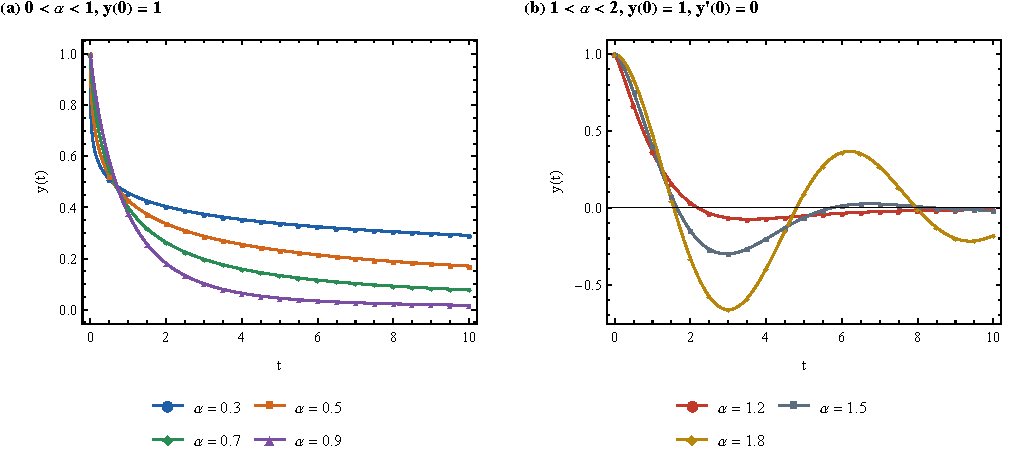
\includegraphics[width=\linewidth]{fig1_mittag_leffler.pdf}
\caption{Relaxation ${}^{C}\!D^{\alpha}y=-y$: exact Mittag-Leffler solutions (lines) and PECE with $N=400$, $M=2$ (markers).}\label{fig:ml}\end{figure}

\begin{figure}[H]\centering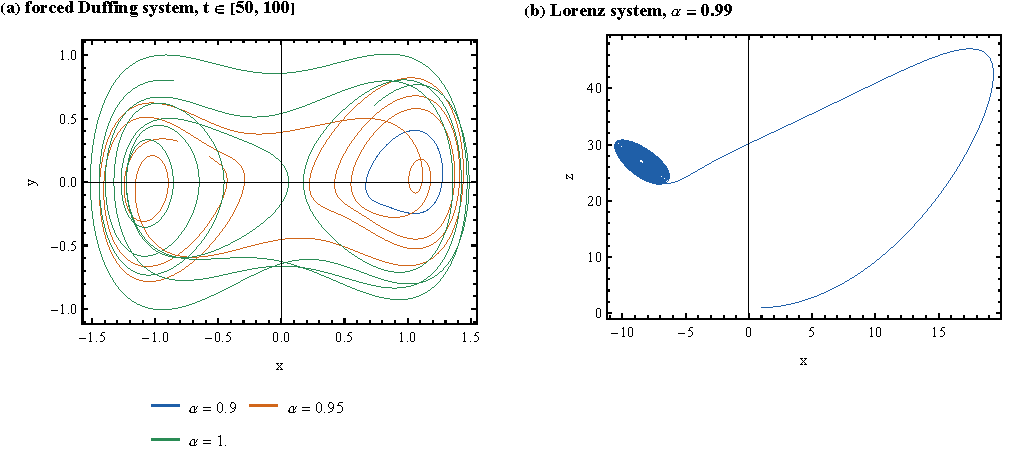
\includegraphics[width=\linewidth]{fig4_applications.pdf}
\caption{Commensurate systems solved with PECE ($M=2$): (a) forced Duffing oscillator for three orders; (b) Lorenz system ($\sigma=10$, $\rho=28$, $\beta=8/3$) with $\alpha=0.99$, $x$--$z$ projection.}\label{fig:app}\end{figure}

\begin{figure}[H]\centering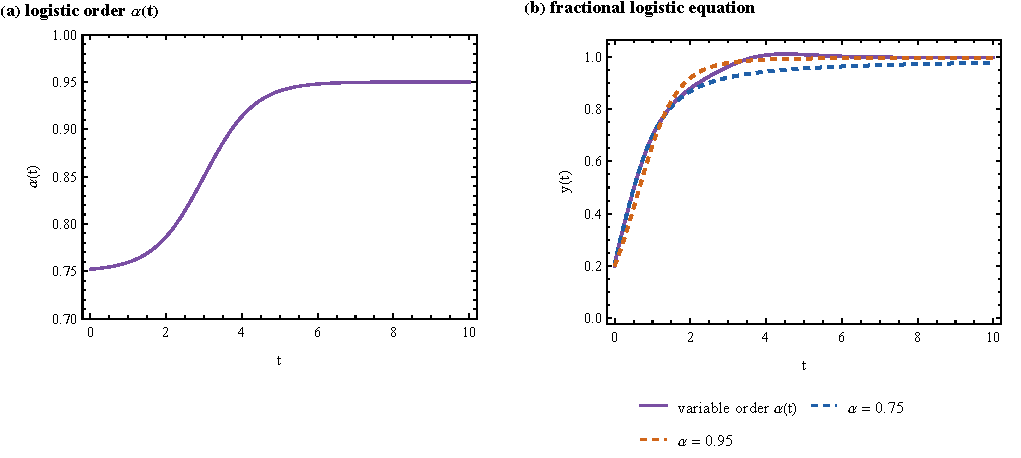
\includegraphics[width=\linewidth]{fig5_variable_order.pdf}
\caption{Variable-order fractional logistic equation: (a) the order $\alpha(t)$; (b) variable-order solution and constant-order solutions ($N=2000$).}\label{fig:vo}\end{figure}

\subsection{Verification}
\textit{Automated tests.} The Wolfram suite \texttt{RunTests.wls} contains \wlTests{} tests, and \wlPassed{} pass on Mathematica \mmaVersion{}; the Python suite contains \pythonTests{} tests, all passing. The tests check convergence orders against Mittag-Leffler solutions and the nonlinear benchmark, systems, variable order, the Gr\"unwald--Letnikov weights, the Strong-FDM and L1 orders, the decrease of the residual, and agreement of 40 reference values with the Python implementation to a relative $10^{-10}$.

\textit{Convergence.} Figure~\ref{fig:conv} and Table~\ref{tab:orders} use the benchmark of Diethelm, Ford and Freed \cite{dff2004}
${}^{C}\!D^{\alpha}y=\tfrac{40320}{\Gamma(9-\alpha)}t^{8-\alpha}-3\tfrac{\Gamma(5+\alpha/2)}{\Gamma(5-\alpha/2)}t^{4-\alpha/2}+\tfrac94\Gamma(\alpha+1)+\big(\tfrac32t^{\alpha/2}-t^4\big)^3-y^{3/2}$, $y(0)=0$ (and $y'(0)=0$ for $\alpha>1$), with exact solution $y=t^8-3t^{4+\alpha/2}+\tfrac94t^{\alpha}$. PECE with one corrector converges with order $1+\alpha$ for $\alpha<1$ (\ordPECEhalf{} at $\alpha=0.5$) and order 2 for $\alpha>1$. Three corrector iterations, the implicit trapezoidal rule and Lubich--BDF2 with starting weights reach order close to 2 for all six values of $\alpha$, and Lubich--BDF1 is first order. The variable-order solver converges with observed order \voOrder{} on the logistic example.

\begin{figure}[H]\centering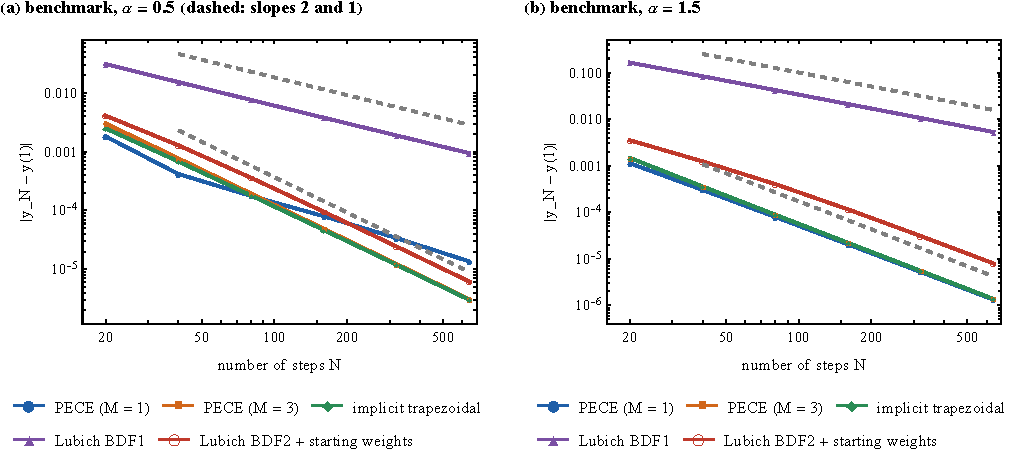
\includegraphics[width=\linewidth]{fig2_convergence.pdf}
\caption{Error at $t=1$ on the Diethelm--Ford--Freed benchmark for the five solvers: (a) $\alpha=0.5$; (b) $\alpha=1.5$.}\label{fig:conv}\end{figure}

\begin{table}[H]\centering\scriptsize\setlength{\tabcolsep}{3pt}
\caption{Error at $t=1$ for $N=640$ and observed order (between $N=320$ and $640$) on the benchmark. For PECE with $M=1$ at $\alpha=0.75$ the error changes sign between the two grids, so the observed order is not meaningful.}\label{tab:orders}
\begin{tabular}{@{}l*{5}{cc}@{}}\toprule
& \multicolumn{2}{c}{PECE, $M=1$} & \multicolumn{2}{c}{PECE, $M=3$} & \multicolumn{2}{c}{trapezoidal} & \multicolumn{2}{c}{Lubich BDF1} & \multicolumn{2}{c}{Lubich BDF2}\\
$\alpha$ & error & order & error & order & error & order & error & order & error & order\\\midrule
\inputrows{../tables/benchmark_orders.tex}
\bottomrule\end{tabular}\end{table}

\textit{Caputo operators.} Figure~\ref{fig:ops}(a) shows that, for $\alpha=0.5$, Strong-FDM is second order for $e^{t}$ and $t^{3.5}$, while L1 has order $2-\alpha=1.5$ and errors one to two orders of magnitude larger. Figure~\ref{fig:ops}(b) shows second order for Strong-FDM on $e^{t}$ for $\alpha=0.3,0.8$ and, with the third-difference stencil, for $\alpha=1.3,1.7$. At the finest grid the error approaches the round-off level of the $h^{-p}$ stencil. For functions whose $p$-th derivative is singular at the origin (such as $t^{\alpha}$-type solutions), the order of Strong-FDM is reduced, and L1 is the more robust operator.

\textit{Residual certificate and cost.} Figure~\ref{fig:res}(a) shows the residual of PECE solutions ($M=3$) of ${}^{C}\!D^{0.5}y=\Gamma(4)t^{2.5}/\Gamma(3.5)+1+t^3-y$, $y(0)=1$ (exact solution $1+t^3$). For $N=640$ the Strong-FDM residual is at most \resMaxSF{}, against \resMaxLone{} with L1, and the solution error is \errMaxRes{}. The residual decreases with $N$ and therefore certifies the computed solution without knowledge of the exact one. All solvers have $O(N^2)$ cost (Figure~\ref{fig:res}(b)); for $N=1600$ a scalar problem takes \timePECE{}~s (PECE), \timeLUB{}~s (Lubich BDF2) and \timeTRAP{}~s (trapezoidal) on a laptop.

\begin{figure}[H]\centering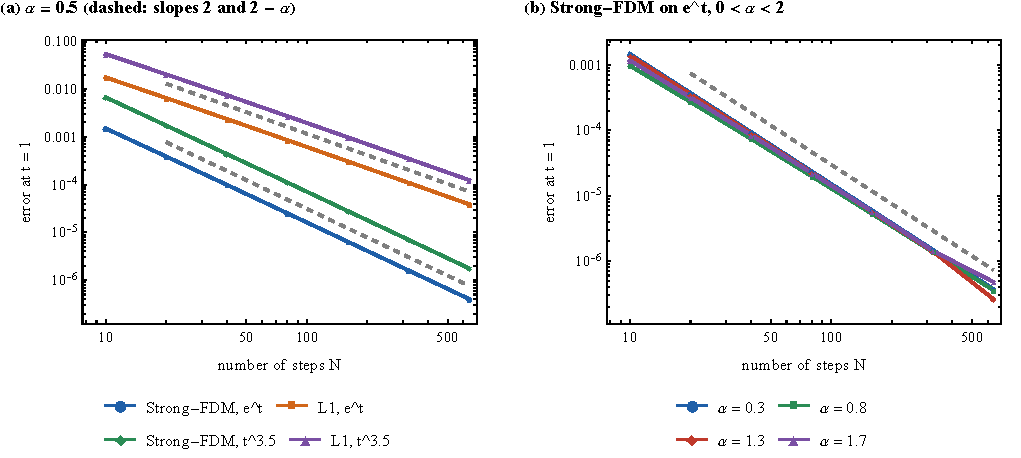
\includegraphics[width=\linewidth]{fig3_caputo_operators.pdf}
\caption{Error at $t=1$ of the discrete Caputo derivative: (a) Strong-FDM and L1 for $\alpha=0.5$; (b) Strong-FDM on $e^t$ for $\alpha=0.3,0.8,1.3,1.7$.}\label{fig:ops}\end{figure}

\begin{figure}[H]\centering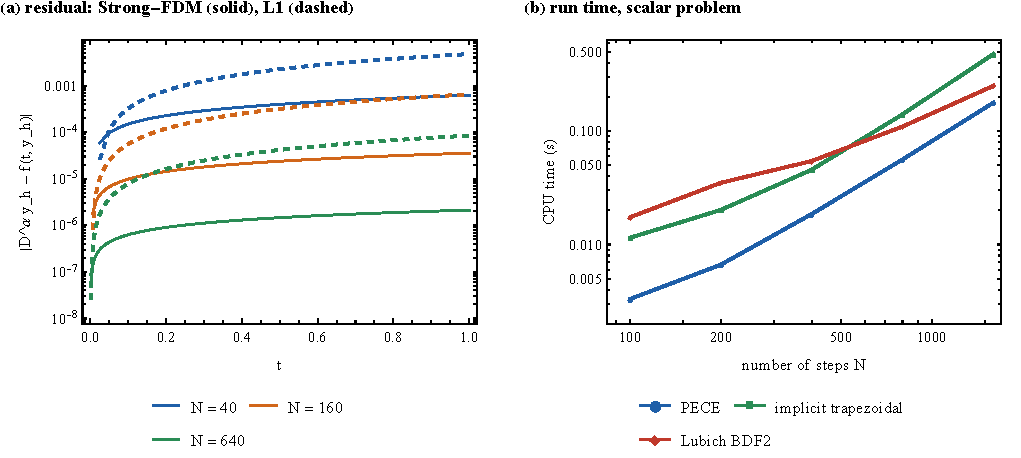
\includegraphics[width=\linewidth]{fig6_residual_and_cost.pdf}
\caption{(a) Residual $|{}^{C}\!D^{\alpha}y_h-f(t,y_h)|$ of PECE solutions for $N=40,160,640$, evaluated with Strong-FDM (solid) and L1 (dashed). (b) Run time versus $N$.}\label{fig:res}\end{figure}

\section{Impact}
The package gives Mathematica users tested solvers for Caputo fractional differential equations, and lets them check a solution in three independent ways: by comparing methods of different construction, by refining the grid, and by the residual certificate. It is intended as a reference tool for the many studies of fractional oscillators, population and epidemic models and chaotic systems, where results are often reported from a single, unverified scheme. Every figure and table in this paper is regenerated by \texttt{RunTests.wls} and \texttt{MakeFigures.wls}, so the verification can be repeated and extended. No claims of existing adoption are made for this initial release.

\section{Conclusions}
FractionalODELab provides PECE, implicit trapezoidal, Lubich convolution-quadrature and variable-order solvers for Caputo fractional differential equations of order $0<\alpha<2$, together with L1 and Strong-FDM discrete Caputo operators. Its convergence orders agree with theory, its results agree with an independent Python implementation, and its residual certificate allows a-posteriori checking of computed solutions.

\textit{Limitations and future work.} The solvers use uniform grids and $O(N^2)$ history sums; fast and sum-of-exponentials convolution, adaptive steps and multi-order systems are not yet implemented. The starting weights of Lubich--BDF2 are limited to four exponents, because larger sets are ill-conditioned \cite{dff2006}; for small $\alpha$ the trapezoidal rule or PECE with several correctors is recommended. The variable-order solver uses the frozen-order product integration for $0<\alpha(t)<1$ and has been verified by self-convergence only. Strong-FDM is second order for smooth functions and has a round-off floor of order $\varepsilon h^{-p}$.

\section*{Availability and reproducibility}
The source code, tests and scripts are available at \url{https://github.com/alvarohumberto/FractionalODELab} under the MIT license. Running \texttt{wolframscript -file mathematica/RunTests.wls} and \texttt{mathematica/MakeFigures.wls} regenerates every figure and table. Appendix~\ref{app:wl} documents the package and lists its source code.
\section*{CRediT authorship contribution statement}
Alvaro H. Salas: Conceptualization, Methodology, Software, Validation, Writing -- original draft, Writing -- review and editing.
\section*{Declaration of competing interests}
The author declares no known competing financial interests or personal relationships that could have appeared to influence the work reported in this paper.
\section*{Funding}
No external funding was received.
\section*{Data availability}
No external data were used. All data shown are generated by the scripts in the repository.

\begin{thebibliography}{99}
\bibitem{podlubny} I. Podlubny, \emph{Fractional Differential Equations}, Academic Press, San Diego, 1999.
\bibitem{diethelmbook} K. Diethelm, \emph{The Analysis of Fractional Differential Equations}, Lecture Notes in Mathematics 2004, Springer, Berlin, 2010.
\bibitem{kilbas} A. A. Kilbas, H. M. Srivastava, J. J. Trujillo, \emph{Theory and Applications of Fractional Differential Equations}, Elsevier, Amsterdam, 2006.
\bibitem{dff2002} K. Diethelm, N. J. Ford, A. D. Freed, A predictor--corrector approach for the numerical solution of fractional differential equations, \emph{Nonlinear Dynamics} 29 (2002) 3--22.
\bibitem{dff2004} K. Diethelm, N. J. Ford, A. D. Freed, Detailed error analysis for a fractional Adams method, \emph{Numerical Algorithms} 36 (2004) 31--52.
\bibitem{dff2006} K. Diethelm, J. M. Ford, N. J. Ford, M. Weilbeer, Pitfalls in fast numerical solvers for fractional differential equations, \emph{Journal of Computational and Applied Mathematics} 186 (2006) 482--503.
\bibitem{lubich1986} C. Lubich, Discretized fractional calculus, \emph{SIAM Journal on Mathematical Analysis} 17 (1986) 704--719.
\bibitem{lubich1988} C. Lubich, Convolution quadrature and discretized operational calculus I, \emph{Numerische Mathematik} 52 (1988) 129--145.
\bibitem{garrappa2015} R. Garrappa, Trapezoidal methods for fractional differential equations: theoretical and computational aspects, \emph{Mathematics and Computers in Simulation} 110 (2015) 96--112.
\bibitem{garrappa2018} R. Garrappa, Numerical solution of fractional differential equations: a survey and a software tutorial, \emph{Mathematics} 6 (2018) 16.
\bibitem{salasstrong} A. H. Salas, Fast evaluation of the Caputo derivative: a strong midpoint-FDM scheme compared with L2, modified L1, and BDF2-CQ, manuscript, 2026.
\bibitem{grigorenko} I. Grigorenko, E. Grigorenko, Chaotic dynamics of the fractional Lorenz system, \emph{Physical Review Letters} 91 (2003) 034101.
\bibitem{petras} I. Petr\'a\v{s}, \emph{Fractional-Order Nonlinear Systems: Modeling, Analysis and Simulation}, Springer, Berlin, 2011.
\bibitem{wolfram} Wolfram Research, Inc., Mathematica, Version 15.0, Champaign, IL, 2026.
\end{thebibliography}

\clearpage
\appendix
\nolinenumbers
\section{Wolfram Language implementation and usage}\label{app:wl}
\subsection{Installation and running}
Download or clone the repository (\url{https://github.com/alvarohumberto/FractionalODELab}) and load the package by file name:
\begin{wlcode}
Get["C:/path/to/FractionalODELab/mathematica/FractionalODELab.wl"]
FOLVersion        (* "0.1.0" *)
\end{wlcode}
The tests, figures and tables are reproduced with
\begin{wlcode}
wolframscript -file mathematica/RunTests.wls       (* 36 tests -> test_report.txt / .csv *)
wolframscript -file mathematica/MakeFigures.wls    (* figures/*.pdf, *.png; tables/*.tex, *.csv *)
\end{wlcode}
or from a notebook with \texttt{Get["\dots/RunTests.wls"]} and \texttt{Get["\dots/MakeFigures.wls"]}. Together they run in about two minutes on a laptop.

\subsection{Calling convention and options}
All solvers take \texttt{f}, a function of $(t,y)$ (pure functions \texttt{-\#2 \&} are convenient), the order \texttt{alpha}, the initial data \texttt{y0} ($y(0)$ for $\alpha\le1$, $\{y(0),y'(0)\}$ for $1<\alpha<2$; vectors for systems) and \texttt{\{T, N\}}. They return \texttt{\{t, y\}}, where \texttt{y} is a list of numbers (scalar case) or of vectors (systems); \texttt{FOLInterpolation} turns it into interpolating functions. Options: \texttt{FOLPECE}: \texttt{"CorrectorIterations"} (1), \texttt{"Implicit"} (\texttt{False}); \texttt{FOLLubich}: \texttt{"Order"} (2), \texttt{"StartingWeights"} (\texttt{True}); Newton-based solvers: \texttt{"Tolerance"} ($10^{-13}$), \texttt{"MaxIterations"} (50); \texttt{FOLCaputoStrongFDM} and \texttt{FOLResidual}: \texttt{"InitialDerivative"} ($u^{(p-1)}(0)$), and \texttt{FOLResidual}: \texttt{"Operator"} (\texttt{"StrongFDM"} or \texttt{"L1"}).

\subsection{Usage examples}
\subsubsection*{Relaxation and comparison with the Mittag-Leffler function}
\begin{wlcode}
{t, y} = FOLPECE[-#2 &, 0.6, 1., {5., 500}, "CorrectorIterations" -> 2];
Max[Abs[y - MittagLefflerE[0.6, -t^0.6]]]               (* maximum error *)
{t, y} = FOLLubich[-#2 &, 1.5, {1., 0.}, {5., 500}];     (* 1 < alpha < 2: y(0) = 1, y'(0) = 0 *)
\end{wlcode}
\subsubsection*{Nonlinear systems}
\begin{wlcode}
duffing = {#2[[2]], -0.15 #2[[2]] + #2[[1]] - #2[[1]]^3 + 0.3 Cos[#1]} &;
{t, xy} = FOLPECE[duffing, 0.95, {0.5, 0.}, {100., 8000}, "CorrectorIterations" -> 2];
ListLinePlot[xy[[4001 ;;]], AspectRatio -> 0.7]           (* phase portrait for t in [50, 100] *)
{t, y} = FOLTrapezoidal[{-100 #2[[1]] + #2[[2]], -#2[[2]]} &, 0.8, {1., 1.}, {1., 200}];  (* stiff *)
\end{wlcode}
\subsubsection*{Variable order}
\begin{wlcode}
al = 0.75 + 0.2/(1 + Exp[-1.5 (# - 3)]) &;
{t, y} = FOLVariableOrderPECE[2 #2 (1 - #2) &, al, 0.2, {10., 2000}];
\end{wlcode}
\subsubsection*{Caputo operators and residual certificate}
\begin{wlcode}
FOLCaputoStrongFDM[Exp, 0.5, 0.01, 100, "InitialDerivative" -> 1.]   (* D^0.5 e^t at t = 0.01 .. 1 *)
FOLCaputoL1[Exp[Range[0., 1., 0.01]], 0.5, 0.01]
f = Gamma[4]/Gamma[3.5] #1^2.5 + 1 + #1^3 - #2 &;
sol = FOLPECE[f, 0.5, 1., {1., 320}, "CorrectorIterations" -> 3];
Max[Abs[FOLResidual[f, 0.5, sol, "InitialDerivative" -> 0.]]]       (* a-posteriori residual *)
\end{wlcode}

\subsection{Package source: \texttt{FractionalODELab.wl}}\label{app:src}
The complete package is listed below; the verification suite and figure scripts are in the \texttt{mathematica/} folder of the repository.
\lstinputlisting[style=wl]{../mathematica/FractionalODELab.wl}
\end{document}
